\documentclass{article}

\usepackage{amsmath}
\usepackage{tikz}
\usepackage{graphicx}

\title{Turing Machine Documentation}
\author{Ryan Peruski, Maria Hernandez}
\date{\today}

\begin{document}

\maketitle
\section{Roles}

\begin{itemize}
    \item Ryan Peruski: Created initial stack design and initial templates for the documentation
    \item Maria Hernandez
\end{itemize}
\section{Definition}
This Turing machine uses the power of the stack to do a simple check for C-code. It checks for correct parenthesis, square bracket, and curly brace
placement. It will accept any code that has correct placement of these characters, and it will reject any code that does not.

\section{States, Transitions, Image}
The Turing machine operates by moving between states and performing transitions on the tape. The states and transitions are labelled as follows:

\begin{itemize}
    \item $Red$ are all the reject states ($q_{reject}$)
    \item $Green$ are all the accept states ($q_{accept}$)
    \item $Blue$ is the Queue's add States
    \item $Yellow$ is the Queue's remove States (1st part: $deletion$)
    \item $Orange$ is the Queue's remove States  (2nd part: $movement$)
    \item $Magenta$ is the Stack with the add states
    \item $Cyan$ is the Stack with the remove states
    \item $Black$ are the initial states to set up the $\#$
\end{itemize}

The transitions can be summarized as follows:
\begin{itemize}
    \item xxxxxx
    \item xxxxxx
\end{itemize}

Finally, the Turing Machine is shown in Figure\ \ref{fig:stackqueue}.
\begin{figure}
    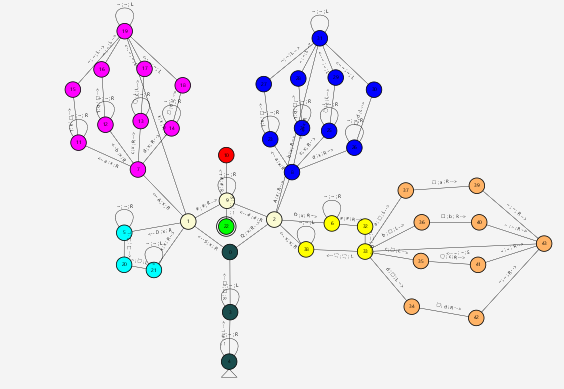
\includegraphics[width=\linewidth]{stackqueue.png}
    \caption{Turing Machine.}\label{fig:stackqueue}
\end{figure}

\section{Instructions}
This Turing Machine can input any C-code (or code in general that uses parenthesis) and it will place left parenthesis on the stack and pop
right parenthesis. If it does not see a parenthesis of the right type or none at all, it will reject. If the code ends with anything on the
stack, it will reject. If the code is empty, it will accept. 

The only thing that the machine will reject on is a $\#$, as this is a marker between the code and the stack.

\section{Examples}
Here are some examples of input and output for the Turing machine:
\begin{itemize}
    \item \begin{verbatim} Input: v[i] = a[i][j];, Output: xxxxxxxxxxxxxxx#qa \end{verbatim}
    \item \begin{verbatim} Input: for (;;) break;, Output: xxxxxxxxxxxxxxx#qa \end{verbatim}
    \item \begin{verbatim} Input: {x = 7}, Output: xxxxx#qa \end{verbatim}
    \item \begin{verbatim} Input: for(i=0;i<v.size();i++) v[i]=2;, Output: xxxxxxxxxxxxxxxxxxxxxxxxxxxxxx#qa \end{verbatim}
    \item \begin{verbatim} Input: v[i] = a[i, Output: INVALID \end{verbatim}
    \item \begin{verbatim} Input: for(;;, Output: INVALID \end{verbatim}
\end{itemize}

\section{Conclusion}
The Turing machine is a powerful tool for performing computations on input tapes. It has applications in computer science, mathematics, and other fields.

\end{document}